\chapter{不变子空间}

\section{不变子空间的定义}
在介绍本节内容前,我们需要首先对算子(operator)这一名词进行解释.
\begin{definition}
	向量空间到其自身的线性映射成为算子.
\end{definition}
以上是《线性代数应该这样学》对于算子的定义,本章中出现算子一词也默认为此含义.
实际上,狭义的算子指从一个函数空间到另一个函数空间(或其自身)的映射,例如
微积分中学习的梯度,散度以及拉普拉斯算子等.本书中采用的是广义的定义,将算子
这一定义延伸至向量空间.

需要注意的是,done right喜欢用抽象的算子作为研究对象,一般的高等代数则更喜欢具象的矩阵,
实际上二者是完全统一的,很多定理虽然用算子描述,实际上也有相应的矩阵版本.因为实际上矩阵$A$可以视为
算子$T\alpha=A\alpha$在自然基下的矩阵,由此可以做到统一.

在我们接下来的叙述中,我们希望将算子在基下的矩阵表示尽可能简单.在下面的内容中,有三个关键概念是
要经常提及的:算子,矩阵以及多项式,接下来的主干内容就是围绕这三者之间的关系展开.我可以在此画一个
三角形,各边连线上的内容大家可以在阅读过程中自己补全.
\begin{figure}[h]
	\centering
	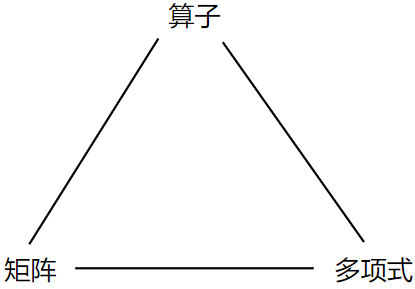
\includegraphics[scale=0.4]{./figs/15/15-1.png}
\end{figure}

我们在上一章中讨论了算子可对角化的充要条件.但事实上存在大量不可对角化
的算子,我们也希望得到其最简单的矩阵表示形式.在定理\ref{可对角化充要条件}
中我们可以看到,$V$上算子$T$可对角化当且仅当$V$可以分解为$T$的特征子空间的
直和:$$V=V_{\lambda_1}\oplus V_{\lambda_2}\oplus\cdots\oplus V_{\lambda_s},$$
其中$\lambda_1,\lambda_2,\cdots,\lambda_s$为$T$的所有不同本征值.我们注意到
$\alpha\in V_{\lambda_i},T\alpha=\lambda_i\alpha\in V_{\lambda_i}$,这启示
我们可以将$V$分解为具有这一性质的子空间的直和来研究矩阵的简化形式.满足这一性质的
空间对于我们的研究非常重要,我们需要给予它一个定义:
\begin{definition}
	设$T\in L(V)$,若$V$的子空间$U$满足$\forall \alpha\in U,T\alpha\in U$,
	则称$U$是$T$的不变子空间,简称为$T$-子空间.
\end{definition}
即不变子空间中的每一个向量在算子作用后仍在这一空间中.为了研究在某一子空间下映射的性质,
我们还需要引入映射的限制的概念:
\begin{definition}
	设$g:A\to B$是一个映射,在$A$的子集$A_0$上定义$f:A_0\to B$满足$f(a)=g(a),\forall a\in A_0$,
	则称$f$为$g$关于集合$A_0$的限制映射,记为$f=g|_{A_0}$.
\end{definition}
即限制映射就是将原映射的定义域进行收缩,但原定义域上的函数值保持不变.
事实上,若映射为线性映射,限制的集合为线性映射的不变子空间,则这一映射限制在这一空间上成为算子,
我们称其为\textbf{限制算子}.

如果$U$是$T$的不变子空间,那么$T$还可以诱导出商空间$V/U$上的一个线性变换$T/U$,满足
$(T/U)(v+U)=Tv+U$,其中$v\in V$,称之为\textbf{商算子}.

这一定义的线性性容易验证,这里需要提及的是合理性(即是否是良定义,或well-defined的).
事实上,对于一个映射,其合理性在于原像集合中的一个元素只能映射到像集中的唯一一个值
(否则不符合映射的定义).商算子的出发空间元素是等价类,因此如果出现$v+U=w+U$但$Tv+U\neq Tw+U$
的情况,这一定义描述的就不是映射,因此不是良定义.但我们可以验证这一映射是良定义的,详见教材106页.
\begin{example}
	设$T\in L(V,W)$,定义$\tilde{T}:(V/(\textup{null }T))\to W$如下:
	$$\tilde{T}(v+\textup{null }T)=Tv.$$

	\textup{(1)}$\tilde{T}$是良定义的,且是$(V/(\textup{null }T))$到$W$上的线性映射;

	\textup{(2)}$\tilde{T}$是单射;

	\textup{(3)}$\textup{range }\tilde{T}=\textup{range }T$;

	\textup{(4)}$V/(\textup{null }T)$同构于$\textup{range }T$.
\end{example}
\begin{example}
	设$T\in L(V)$,证明:

	\textup{(1)}$T/(\textup{range }T)=0$;

	\textup{(2)}$T/(\textup{null }T)$是单的当且仅当$\textup{null }T\cap\textup{range }T=\{0\}$.
\end{example}
教材例5.3给出了四个常见的不变子空间的例子,分别是两个平凡子空间和映射的像与核.教材8.20还给出了$p$
为多项式时,$\textup{null }p(T)$和$\textup{range }p(T)$也为$T$的不变子空间.但有时我们可能会遇到
更为复杂的情形,如下面的例子:
\begin{example}
	设$V$是$n$维复向量空间,$T\in L(V)$,若$T$有$n$个互异的本征值,求$T$的所有不变子空间的个数.
\end{example}
\begin{example}
	设$\mathbf{F}$为一数域,算子$T$定义为
	$$T(a,b)=(a,b)\begin{pmatrix}
		1 & -1 \\ 2 & 2
	\end{pmatrix},$$证明:

	\textup{(1)}当$\mathbf{F}=\mathbf{R}$时,$\mathbf{R}^2$无$T$的非零真不变子空间;

	\textup{(2)}当$\mathbf{F}=\mathbf{C}$时,$\mathbf{C}^2$有$T$的非零真不变子空间.
\end{example}
除此之外,还有一些问题我们将在讨论若当标准形时进行讨论.

\section{特征值与特征向量}
从本章起,我们主要研究线性变换(而非一般线性映射)和方阵的性质.
\subsection{特征值与特征向量的定义与求解}
首先介绍线性变换和矩阵的特征值与特征向量的概念:
\begin{definition}
	设$\sigma$是线性空间$V(\mathbf{F})$上的一个线性变换,如果存在数$\lambda\in\mathbf{F}$
	和非零向量$\xi\in V$使得$\sigma(\xi)=\lambda\xi$,则称数$\lambda$为$\sigma$的一个特征值,
	并称非零向量$\xi$为$\sigma$属于其特征值$\lambda$的特征向量.
\end{definition}
必须注意特征向量为非零向量,否则零向量对任意$\lambda$都满足上面定义,从而失去“特征”的含义.
但是特征值可以为0,此时实际上就是线性变换的零空间.

特征值与特征向量的几何意义在于,某一线性变换的特征向量在经过变换后得到的向量与原先向量共线.

我们称关于同一个特征值$\lambda$的所有特征向量构成的集合记为$V_\lambda=\{\xi\ |\ \sigma(\xi)=\lambda\xi,\xi\in V\}$,
称为$\sigma$关于其特征值$\lambda$的特征子空间.
\begin{example}
	证明:$V_\lambda$是$V$的子空间.
\end{example}
实际上,$\sigma(\xi)=\lambda\xi$等价于$(\lambda I-\sigma)(\xi)=0$,故特征子空间就是线性变换
$\lambda I-\sigma$的核,核中必有非零向量(特征向量非零),故$\lambda I-\sigma$在$\lambda$为特征值时
必不满秩,故我们可以通过$|\lambda E-A|=0$求解特征值,其中$A$为$\sigma$在某组基下的矩阵.
对于特征向量的求解,求出$(\lambda E-A)X=0$的非零解就是特征向量在基下的坐标.

上面是线性变换的特征值与特征向量的定义,我们在考试中更一般地会遇到下述矩阵的特征值与特征向量的定义:
\begin{definition}
	设矩阵$A\in M_n(\mathbf{F})$,如果存在数$\lambda\in\mathbf{F}$和非零向量$X\in\mathbf{F}^n$使得
	$AX=\lambda X$,则称数$\lambda$为$A$的一个特征值,称非零向量$X$为$A$属于其特征值$\lambda$的特征向量.
\end{definition}
\begin{example}
	设$A=\begin{pmatrix}
		1 & -1 & 0 \\ 2 & 0 & 1 \\ 1 & a & 0
	\end{pmatrix}$,且存在非零向量$\alpha$使得$A\alpha=2\alpha$,求$\alpha$.
\end{example}
下面我们说明这两个定义的关系.实际上,假设$A$是$\sigma$在基$\alpha_1,\cdots,\alpha_n$下的表示矩阵,且
$\xi=(\alpha_1,\cdots,\alpha_n)X$,我们有
\begin{align*}
	\sigma(\xi)=\lambda\xi &\Leftrightarrow \sigma(\alpha_1,\cdots,\alpha_n)X=\lambda(\alpha_1,\cdots,\alpha_n)X \\
						   &\Leftrightarrow (\alpha_1,\cdots,\alpha_n)AX=(\alpha_1,\cdots,\alpha_n)(\lambda X) \\
						   &\Leftrightarrow AX=\lambda X
\end{align*}
因此$\lambda$同时是线性变换和矩阵的特征值,与基的选取无关,但$X$与基的选取有关.

我们在之前已经分析了求解特征值的方法,即求解$f(\lambda)=|\lambda E-A|$的根. 我们称其为矩阵$A$的特征多项式.
其$k$重根称为$k$重特征值(或称代数重数),对应的特征子空间维数称几何重数.

我们展开特征多项式得到以下定理:
\begin{theorem}
	对于$n$级矩阵$A=(a_{ij})$,记
	$$f(\lambda)=|\lambda E-A|=a_0\lambda^n+a_1\lambda^{n-1}+\cdots+a_{n-1}\lambda+a_n.$$
	则$a_0=1$,$a_n=(-1)^n|A|$,且$a_k$等于所有$k$级主子式之和乘以$(-1)^k$.
\end{theorem}
这一定理的证明无需掌握,并且关于特征多项式的进一步讨论也将在线性代数II中涉及.这里我们主要掌握两个特例,
即由韦达定理,我们有$\sum\limits_{i=1}^{n}\lambda_i=\sum\limits_{i=1}^{n}a_{ii}$,
$\prod\limits_{i=1}^{n}\lambda_i=|A|$,
即特征值按重数求和为矩阵的迹(即矩阵对角线元素之和),特征值按重数求积为矩阵行列式.
这一结论在解决某些问题时有一定作用.

\subsection{特征值的基本性质}
关于特征值,我们有如下基本性质,证明较为基本,可以自行完成:

设$\lambda$是线性空间$V(\mathbf{F})$上的线性变换$\sigma$的特征值,$\xi$是$\sigma$属于$\lambda$的特征向量,则

1. $k\lambda$是$k\sigma$的特征值,$\lambda^m$是$\sigma^m$的特征值,且$\xi$仍是相应特征向量.

2. 若$f(x)=a_nx^n+a_{n-1}x^{n-1}+\cdots+a_1x+a_0$是$\mathbf{F}$上的多项式,则$f(\sigma)(\xi)=f(\lambda)\xi$.

3. 设$\lambda$是$n$阶矩阵$A$的特征值,$A$可逆,则$\lambda^{-1}$是$A^{-1}$的特征值,$|A|\lambda^{-1}$是$A$的伴随矩阵
$A^*$的特征值,且特征向量不变.
\begin{example}
	回答以下问题:

	\textup{(1)}设$A$为三阶矩阵,$A^2-A-2E=O$,$|A|=2$,求$|A^*+3E|$\textup{;}
	
	\textup{(2)}设$A$为三阶矩阵,其特征值为$1$,$-2$,$-1$,求$|A|$,$A^*+3E$的特征值,$(A^{-1})^2+2E$的特征值
	以及$|A^2-A+E|$\textup{;}
	
	\textup{(3)}设$\alpha=(1,0,-1)^\mathrm{T}$,且$A=\alpha\alpha^\mathrm{T}$,求$|6E-A^n|$\textup{;}
	
	\textup{(4)}设$A$为三阶矩阵,其特征值为$-1$,$-1$,$5$,求$A_{11}+A_{22}+A_{33}$\textup{;}
	
	\textup{(5)}设$A$为三阶实对称矩阵,$A^2=A$且$r(A)=2$,求$|A+2E|$.
\end{example}

下面一个例子也是重要的结论,实际上在行列式专题已给出类似结论,但我们现在从特征值角度考虑这一结论:
\begin{example}
	回答以下两个问题:
	
	\textup{(1)}设$A,B$均为$n$阶矩阵,证明:$\lambda\neq 0$是$AB$的特征值,则$\lambda$也是$BA$的特征值\textup{;}
	
	\textup{(2)}设$A\in M_{m\times n}(\mathbf{C}),B\in M_{n\times m}(\mathbf{C})$,证明:
	$$\begin{pmatrix}
		AB & O \\ B & O
	\end{pmatrix}\sim\begin{pmatrix}
		O & O \\ B & BA
	\end{pmatrix},$$
	并由此推出$AB$和$BA$非零特征值相同,且$m=n$时有$|\lambda E-AB|=|\lambda E-BA|$.
\end{example}
不难发现(2)是(1)的推广.下面这一例子也是一些经典的结论,应当熟悉.
\begin{example}
	对下列矩阵$A$的特征值,能做出怎样的断言?
	
	\textup{(1)}$A$可逆/$A$不可逆/$E+A$可逆/$4E+A$不可逆\textup{;}
	
	\textup{(2)}$\det(E-A^2)=0$\textup{;}
	
	\textup{(3)}$AA^\mathrm{T}=A^\mathrm{T}A=E$(正交)/$A^2=E$(对合)/$A^2=A$(幂等)/$A^k=0$(幂零)\textup{;}
	
	\textup{(4)}$A=\lambda_0E+B$($\lambda_0$为常数,且已知$B$的$n$个特征值为$\lambda_1,\lambda_2,\cdots,\lambda_n$)\textup{;}
	
	\textup{(5)}$A$为对角块矩阵,即$A=\begin{pmatrix}
		A_1 &  &  &  \\  & A_2 &  &  \\  &  & \ddots &  \\  &  &  & A_m
	\end{pmatrix}$(与线代$\textup{II}$中不变子空间有关).
\end{example}
在上一小节我们讨论了特征值之和为迹的事实,实际上关于迹以及相关的幂零矩阵的讨论在专题三中已有涉及,
现在可以回过头去再看一些性质的证明.除此之外,我们还可以给幂零矩阵一个等价的定义:
\begin{theorem}
	一个方阵为幂零矩阵当且仅当其所有特征值均为$0$.
\end{theorem}
这一定理“仅当”部分证明比较基本,只需用到上述某一特征值性质即可,但“当”的部分无需掌握证明,需要用到线性代数II的
哈密顿-凯莱定理(事实上很多更进一步的讨论都要基于这一定理).
\subsection{特征向量的基本性质}
这一部分的定理与下一节中可对角化的等价条件直接相关,实际上有了本节的定理,可对角化条件是很显然的.
\begin{theorem}
	线性映射$\sigma$的不同特征值$\lambda_1,\cdots,\lambda_m$对应的特征向量$\xi_1,\cdots,\xi_m$线性无关.
\end{theorem}
\begin{theorem}
	线性映射$\sigma$的不同特征值$\lambda_1,\cdots,\lambda_m$对应的特征子空间$V_{\lambda_1},\cdots,V_{\lambda_m}$的和是直和,
	即$\dim(V_{\lambda_1}+V_{\lambda_2}+\cdots+V_{\lambda_m})=\sum_{j=1}^{m}\dim V_{\lambda_j}$.
\end{theorem}
以上两个定理的证明可以参考教材定理7.7及其推论,实际上二者等价,只需证出其中一个,另一个就是显然的.
两个定理有如下推论:

1. 若$\lambda_1,\cdots,\lambda_m$是线性映射$\sigma$互异的特征值,则$V_{\lambda_i}\cap\sum\limits_{j\neq i}V_{\lambda_j}=\{0\}
(i=1,\cdots,m)$,则一个特征向量不能属于多个特征值.这一推论来源于直和的一个等价条件,专题一的习题中有涉及.

2. $\sigma$的不同特征值$\lambda_1,\cdots,\lambda_m$对应的特征子空间$V_{\lambda_1},\cdots,V_{\lambda_m}$的基向量
合在一起构成的向量组线性无关,且是$V_{\lambda_1}+V_{\lambda_2}+\cdots+V_{\lambda_m}$的基.

接下来这个定理说明了代数重数和几何重数之间的关系:
\begin{theorem}
	$n$维线性空间$V(\mathbf{F})$的线性变换$\sigma$的每个特征值$\lambda_i$的重数(代数重数)大于等于其特征子空间$V_{\lambda_i}$的维数
	(几何重数).
\end{theorem}
这一定理的证明比较复杂,版本也很多,有兴趣的同学可以了解.

\vspace{2ex} 
\centerline{\heiti \Large 内容总结}

\vspace{2ex} 

\centerline{\heiti \Large 习题}
\vspace{2ex} 
{\kaishu }
\begin{flushright}
    \kaishu

\end{flushright}
\centerline{\heiti A组}
\begin{enumerate}
	\item 
\end{enumerate}
\centerline{\heiti B组}
\begin{enumerate}
	\item 
\end{enumerate}
\centerline{\heiti C组}
\begin{enumerate}
	\item 
\end{enumerate}